\chapter{Fundamento teórico y materiales empleados} \label{cap: fundamento_teorico}
En este capítulo se presentarán aquellos conceptos esenciales para comprender el funcionamiento de este proyecto. La intención de este capítulo es hacer una presentación sencilla y fácil de comprender de todos los actores involucrados, para una descripción más en detalle se ha elaborado a modo de apéndice una wiki disponible en el \href{\linkrepositorio}{repositorio de GitHub asociado} \cite{repo_github_TFM_MiguelLerinAlonso}. 

\section{Fundamento teórico}
\subsection{Robot colaborativo}
Un robot colaborativo (o \textit{cobot} en el argot especializado) es un tipo de robot industrial enfocado a trabajar de forma segura y eficiente siempre en compañía de operarios humanos. Es decir el robot y los operadores comparten un entorno físico real en el que interactúan mutuamente y donde debe prevalecer siempre la seguridad del operario. 

Los robots industriales comunes se diseñan para trabajar en tareas repetitivas de alta velocidad y precisión, es decir, resultan idóneos para operaciones especializadas. Estos robots también pueden sostener grandes cargas durante periodos prolongados de tiempo, motivo por el que siempre cuentan con una separación física entre su entorno y el operario como puede ser una barrera de seguridad. La programación de este tipo de robots a menudo viene definida por el fabricante en un entorno cerrado y enfocado a tareas sencillas. Estos motivos han hecho que se les considere equipos destinados a proyectos con tareas claramente definidas en las raramente existan variaciones respecto del modelo original. Es decir, se necesita disponer en todo momento de operarios e ingenieros especializados programando trayectorias in-situ, lo que supone una inversión en tiempo y costes a tener en cuenta.

Los robots colaborativos suponen una alternativa más segura para entornos donde se requiere programar varias tareas en poco tiempo. La premisa de este tipo de manipuladores es la flexibilidad dentro de su entorno físico. Es decir, pese a que se desplazan a velocidades menores que un robot convencional o su carga máxima es más limitada, su diseño ligero y compacto resulta perfecto para un trabajo mano a mano con el operario. Este enfoque permite que se realicen tareas versátiles que no impliquen un riesgo significativo.

En la Figura \ref{fig:comparativa_robots} se muestra una comparativa resumen de ambos equipos.
\begin{figure}[h!]
\centering
    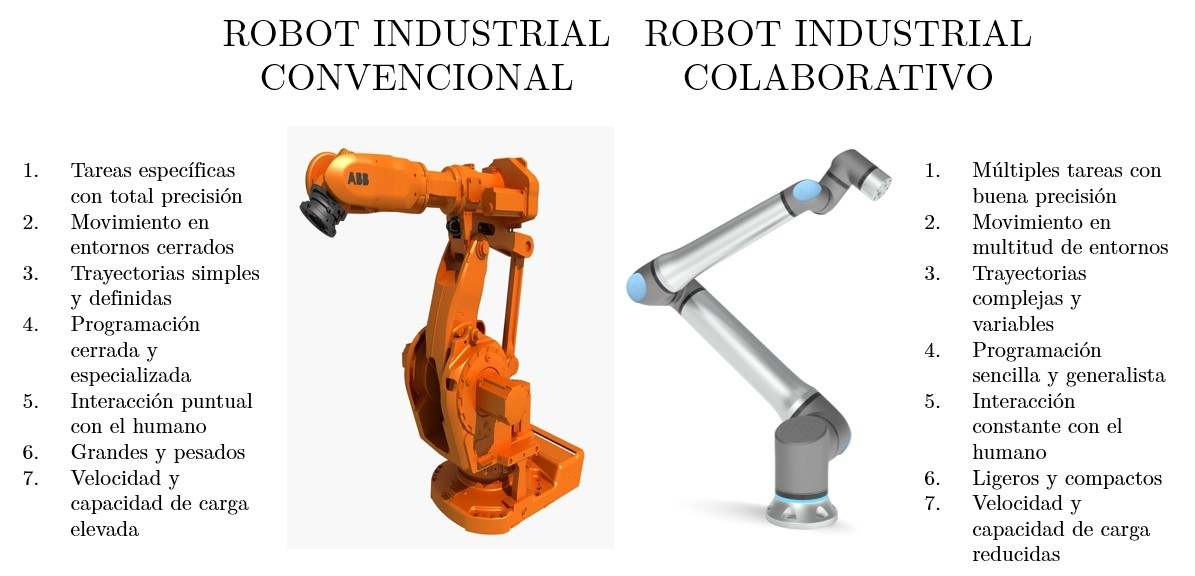
\includegraphics[scale=0.5]{figuras/comparativa_robots_v2.jpg}
    \caption{Comparativa de robots industriales}
    \label{fig:comparativa_robots}
\end{figure}

\subsubsection*{Cobot UR10}
En este trabajo se ha optado por emplear un robot colaborativo UR10 de la marca Universal Robots. Se ha considerado que este equipo resulta ideal para la iniciación en entornos de fabricación aditiva robotizada al poder operar con velocidades reducidas y permitir realizar multitud de iteraciones en poco tiempo. También se ha tenido en cuenta la necesidad de implementar correcciones rápidas de forma directa sin entrañar grandes riesgos para el usuario.

 Las características técnicas de este modelo se muestran en la tabla \ref{tab:caracteristicas_UR}. Existen parámetros cuyo valor es inherente a la unidad utilizada y tuvieron que medirse en el laboratorio en trabajos previos \cite{TFM_SanchoAmparo}.

\begin{table}[h!]
    \begin{subfigure}[h!]{0.45\textwidth}
        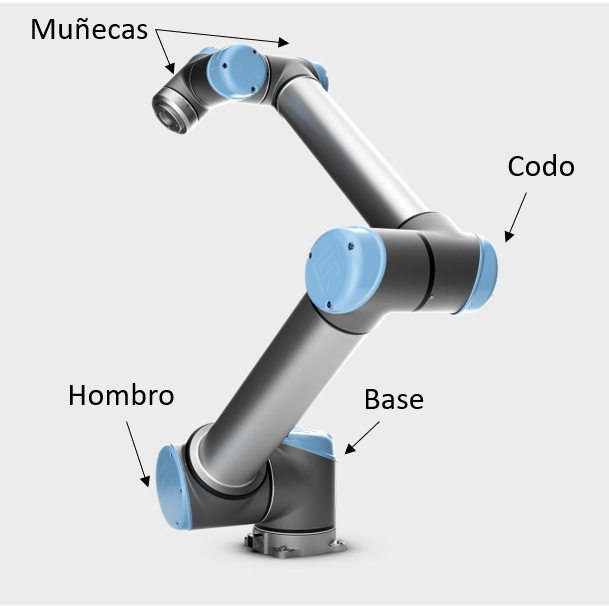
\includegraphics[scale=0.5]{figuras/articulaciones_UR.png}
        %%\caption{Articulaciones del UR}
        \label{fig:articulaciones_UR}
    \end{subfigure}
    \hfill
    \begin{subfigure}[h!]{0.7\textwidth}
        \begin{tabular}{|l|r|}
            \hline
            Carga máxima & 10 kg \\
            \hline
            Alcance máximo & 1300 mm \\
            \hline
            Giro de articulaciones & ± 360º \\
            \hline
            Grados de libertad & 6 \\
            \hline
            Huella & 190 mm \\
            \hline
            Temperatura de trabajo & 0-50 ºC \\
            \hline
            Repetibilidad & ± 0.1 mm \\
            \hline
            Error de trayectoria \footnote{Medido en el laboratorio} & ± 0,2 mm \\
            \hline
            Velocidad de giro de base y hombro & 120 º/s \\
            \hline
            Velocidad de giro de codo y muñeca & 180 º/s \\
            \hline
        \end{tabular}
        %%\caption{Valores característicos}
        \label{tab:caracteristicas_UR_tabla}
    \end{subfigure}
    \caption{Características del UR10 \cite{UR_Technical_Specs}}
    \label{tab:caracteristicas_UR}
\end{table}


\subsection{Cinemática del robot}
Es el campo de estudio del movimiento del robot y la posición de sus articulaciones. En este campo se tiene un especial interés no solamente en el conjunto de poses que le permiten alcanzar al robot un punto del espacio cartesiano, si no también en el comportamiento de sus sensores y actuadores con el transcurso del tiempo. 

No se tienen en cuenta las fuerzas y torques aplicados por el robot para mantener su posición o para manipular algún elemento. El acceso de estos parámetros suele estar únicamente abierto para el fabricante, lo que es de especial utilidad para enfocarse en la labor de cálculo y trazado de trayectorias por parte del usuario.

En el estudio de la cinemática, se ha de tomar siempre un punto de referencia que sirva para la definición de trayectorias, velocidades y aceleraciones que se desea efectuar. Normalmente se suele tomar como convenio el \acrshort{TCP} del robot (también llamado \textit{end-effector} en \href{https://hades.mech.northwestern.edu/images/7/7f/MR.pdf}{literatura especializada de referencia} \cite{Modern_Robotics}). La definición del \acrshort{TCP} pasa por efectuar una serie de transformaciones entre varios marcos de referencia utilizando herramientas matemáticas como las matrices de traslación-rotación (véase como ejemplo la expresión \ref{eq: Ejemplo_matriz_TR}). 

\begin{equation}
\begin{gathered}
    \textbf{TR} =
    \begin{bmatrix}
    1 & 0 & 0 & p_x \\
    0 & 1 & 0 & p_y \\
    0 & 0 & 1 & p_z \\
    0 & 0 & 0 & 1 
    \end{bmatrix}
    \label{eq: Ejemplo_matriz_TR}
\end{gathered}
\end{equation}
\begin{equation*}
\text{Ejemplo de matriz de traslación-rotación}
\end{equation*}

La cinemática busca relacionar dos interpretaciones del espacio con las que debe operar el robot en todo momento:
\begin{itemize}
    \item \textbf{Interpretación cartesiana:} Es la definición de un punto en el espacio a través de tres coordenadas posición (XYZ normalmente) y tres de rotación (ángulos de Euler $\alpha\beta\gamma$)\cite{euler_agle_formulas}. No existe un convenio claro para definir las rotaciones, por lo que existen otras herramientas igualmente válidas como los ángulos aeronáuticos de Tait-Bryan \textit{Roll, Pitch y Yaw} \cite{quaternions_applications} o los \textit{cuaterniones} \cite{Quaternion_Algebra}. Para todas estas herramientas ya existen métodos de conversión bien definidos y fiables \cite{quaternions_and_Euler_Angles}.

    \item \textbf{Interpretación articular:} Es la medida del desplazamiento que debe efectuar el robot para situar su \acrshort{TCP} en el punto destino. Este desplazamiento se mide en referencia al movimiento que debe efectuar cada articulación.
\end{itemize}

Para establecer la relación entre ambas representaciones del espacio, se utilizan las ecuaciones de la cinemática directa y la cinemática inversa. La Figura \ref{fig: comparacion cinematicas} muestra a modo conceptual el enfoque de cada cinemática.

\begin{itemize}
    \item \textbf{Cinemática directa:} Define la posición y orientación del \acrshort{TCP} del robot en el espacio cartesiano a partir de una configuración articular concreta. 

    \item \textbf{Cinemática inversa:} Define los valores de desplazamientos articulares que debe tomar el robot para situar su \acrshort{TCP} en unas posiciones cartesianas de entrada. La solución de este problema no es única y se aborda mediante dos posibles métodos:
        \begin{enumerate}
            \item \textbf{Método geométrico:} Es el más conveniente para robots con un número reducido de \acrshort{DOF}. El enfoque que se suele tomar es el de plantear las ecuaciones de la cinemática directa y despejar de ahí las variables articulares en función de las cartesianas.
            \item \textbf{Cambio entre sistemas de referencia:} Se emplean diferentes métodos numéricos para obtener la matriz de traslación-rotación que define relaciona diferentes sistemas de referencia ubicados en el \acrshort{TCP}, la base del robot, la herramienta e incluso entre los diferentes eslabones. Este método es el más adecuado para un gran número de \acrshort{DOF} por ser fácil de programar y permitir implementar distintos algoritmos de cálculo.
        \end{enumerate}
\end{itemize}

\begin{figure}[h!]
    \centering
    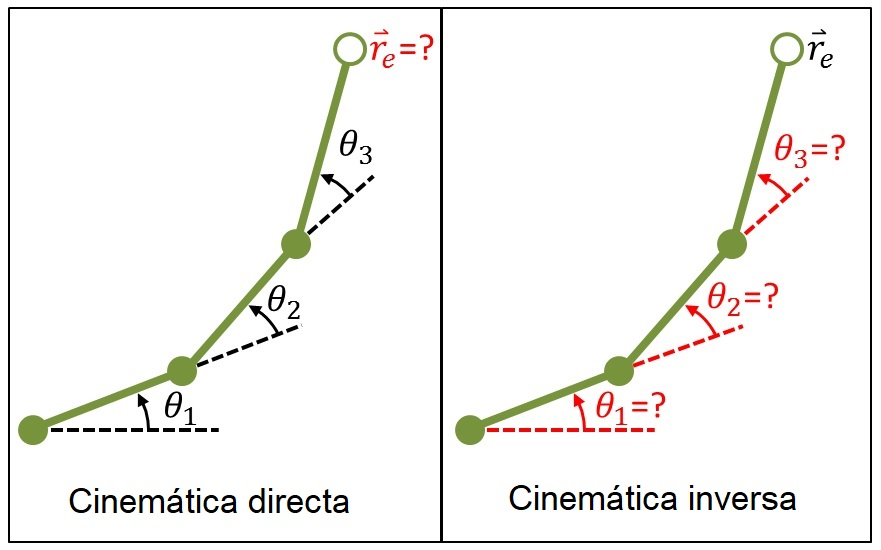
\includegraphics[scale=0.4]{figuras/ik_vs_fk.jpg}
    \caption{Comparación entre cinemáticas \cite{Najam_R_Syed_kinematics_webpage}}
    \label{fig: comparacion cinematicas}
\end{figure}

\subsection{ROS2} \label{section: presentacion ROS2}
ROS2 es un entorno de trabajo software proveniente de \acrshort{ROS}. Se trata un conjunto de librerías e implementaciones software que permite el desarrollo de aplicaciones robóticas a partir de código escrito en lenguajes más generalistas como C++ o Python. De este modo, el usuario puede prescindir de un conocimiento extenso en las implementaciones software del propio robot y centrarse en otras labores como el control de sensores o el cálculo de trayectorias. 

ROS2 sigue los principios fundamentales de su antecesor, pero también implementa ciertas mejoras como:
\begin{itemize}
    \item Soporte multiplataforma entre diferentes lenguajes de programación
    \item Interfaz nativa para sistemas operativos corridos en tiempo real
    \item Mayor modularización entre nodos y paquetes
    \item Implementación de mensajes más flexibles y con comunicación directa ente nodos gracias a protocolos \acrshort{DDS}
\end{itemize}

En este trabajo se ha implementado un sistema de trazado e implementación de trayectorias basado en ROS2 en el robot UR10. Este sistema además es capaz de enviar diversos mensajes entre diferentes nodos y comunicarse con otros equipos de la estación. 

Las siguientes líneas buscan explicar las principales diferencias en el entorno construido con ROS2 frente a uno que implemente \acrshort{ROS}. Si es necesario consultar conceptos básicos de programación en este tipo de entorno, se recomienda consultar la documentación oficial \cite{ROS2_docu_humble} o la \href{\linkrepositorio}{wiki del  repositorio de este proyecto} \cite{repo_github_TFM_MiguelLerinAlonso}.

\begin{itemize}
    \item \textbf{Estructura básica}\\
    \acrshort{ROS} es un entorno de programación robotizada centralizado, es decir, es necesario definir un nodo maestro del que dependerán el resto de nodos. En ROS2 no es necesario definir un único nodo que sirva como base de la jerarquía, el sistema prima la modularización de código. 

    En ROS2, cada vez que se invoca un nuevo nodo en la red, éste es el responsable de avisar al resto de su presencia y de establecer las comunicaciones pertinentes con el resto de módulos. La Figura \ref{fig:Comparacion_ros_ros2} muestra una comparativa entre la estructura de archivos de un proyecto en ROS o otro en ROS2.
    
    \item \textbf{Comunicación entre nodos}\\
    Siguiendo la línea anterior, la capa de transporte de mensajes entre nodos también se ha visto modificada. ROS utilizaba una versión del protocolo \acrshort{TCP/IP} -conocida como TCPROS- que se había modificado de forma específica para cada tipo de comunicación entre nodos. Este enfoque traía problemas de compatibilidad y escalamiento entre tareas, reduciendo la ejecución y compilación del código en el largo plazo o en sistemas operativos en tiempo real.

    Para solventar esta problemática se optó por implementar un \textit{framework} de arquitectura publicador/suscriptor que sirviese como base para escalafones de un mayor nivel de abstracción como cliente/servidor o acción/cliente. Este \textit{framework} se llama \acrshort{DDS} \cite{ROS2_DDS} y se caracteriza por su prioridad en la calidad del mensaje. Es decir, se define un mensaje básico que puede ser interpretado por cualquier objeto de ROS2 y posteriormente se pueden añadir nuevos atributos accesibles al resto de nodos.
    
    \item \textbf{Sistema de compilado}\\
    Cualquier proyecto compilado necesita de un sistema que (1) elabore los ejecutables de forma automática y (2) pueda enlazar las distintas dependencias entre clases y librerías. ROS utiliza Catkin y resulta ideal para proyectos jerarquizados en los que es necesario definir un nodo principal desde el que dependen todas las funcionalidades. No obstante, al ser un sistema que construye archivos de compilación individual -como CMake \cite{documentacion_CMake}, en el que se basa-, Catkin no permite el la compilación entre varias plataformas, por lo que no resulta una buena opción en caso de integrar varias librerías escritas en Python, Java o C++.

    Por su parte Ros1 utiliza \textit{colcon}. Colcon pretende ser más modular y flexible extendiendo la estructura del proyecto gracias a la implementación de dependencias mediante ficheros \acrshort{YAML}. El uso de este tipo de ficheros resulta común a multitud de lenguajes y es más sencillo para el intérprete humano. De este modo se compila un único proyecto que integre diversos paquetes escritos en varios lenguajes en cuestión de segundos.
\end{itemize}

\begin{figure}[h!]
    \centering
    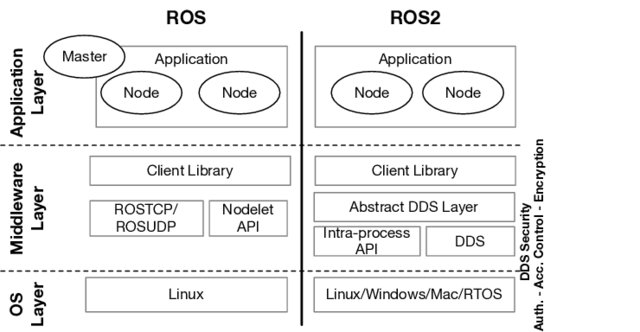
\includegraphics[scale=1.25]{figuras/Comparacion_ros_ros2.jpg}
    \caption{Comparativa entre capas software de ROS y ROS2 \cite{Mazzeo_2020}}
    \label{fig:Comparacion_ros_ros2}
\end{figure}


\subsection{RVIZ}
RViz \cite{guia_RViz} es una herramienta de visualización tridimensional dentro del ecosistema de ROS2. Permite a los desarrolladores y usuarios visualizar y analizar datos relacionados con robots de manera interactiva y en tiempo real. 

Una de sus principales ventajas radica en su capacidad para mostrar modelos 3D de robots basados en archivos \acrshort{URDF} \cite{web_defincion_URDF}, lo que facilita la comprensión de la estructura y la configuración del robot. Además, RViz ofrece una amplia gama de herramientas y accesorios que permiten personalizar la visualización según las necesidades específicas del usuario, desde representación de sensores y actuadores hasta la planificación de trayectorias o la simulación de robots en entornos virtuales.

Las herramientas RViz más empleadas en este trabajo han sido aquellas relacionadas con:
\begin{itemize}
    \item Virtualizar un entorno de trabajo real para implementar un modelo de cálculo de trayectorias que evite colisiones.
    \item Simulación de trayectorias y corrección de errores
    \item Descripción del robot mediante archivo \acrshort{URDF}
    \item Definir sistemas de coordenadas relativos entre diferentes componentes del robot
\end{itemize}

La Figura \ref{fig:entorno_virtual_rviz} muestra el entorno de trabajo de este proyecto virtualizado con ayuda de Rviz. Nótese que de forma análoga a la Figura \ref{fig: estacion_NPAM_sin_estruxor} se han incluido otros elementos complementarios al robot como la mesa de operación o el soporte para el sensor láser.

\begin{figure}[h!]
    \centering
    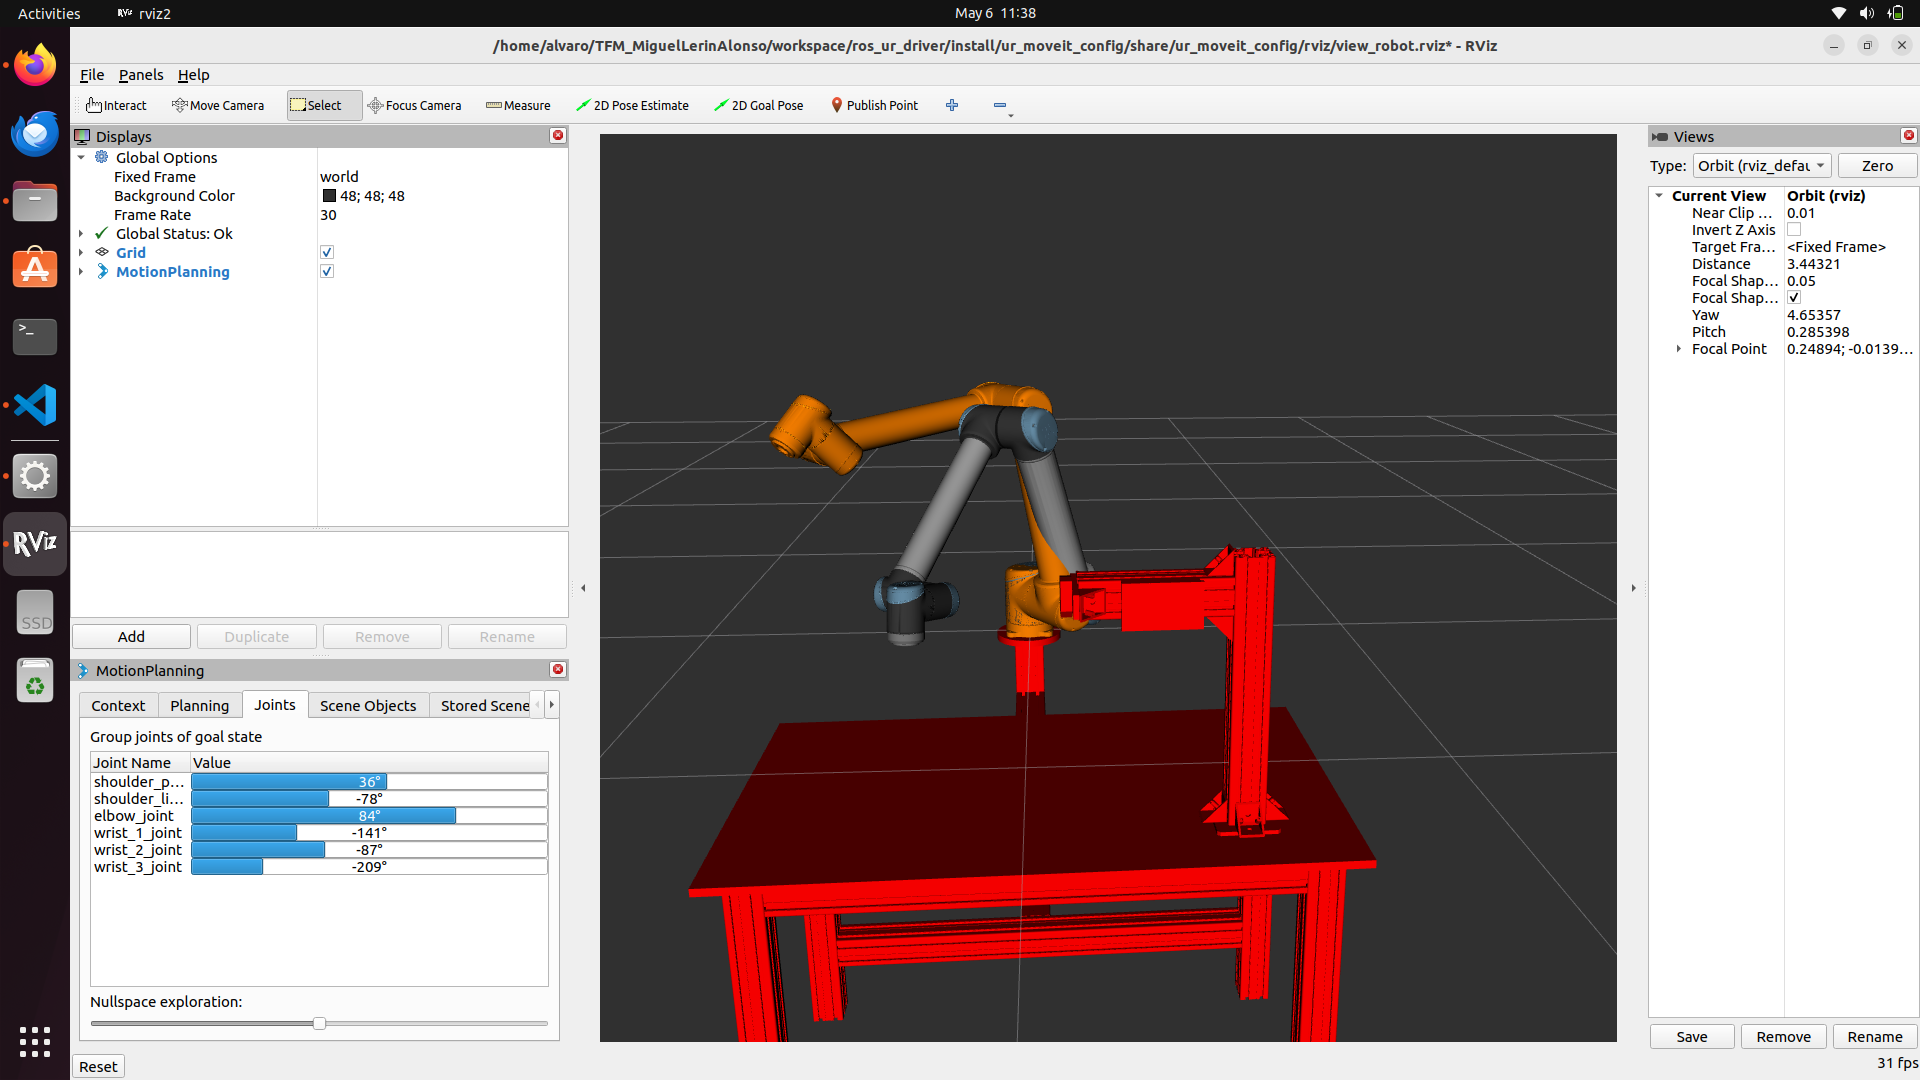
\includegraphics[scale=0.15]{figuras/entorno_virtual_rviz.png}
    \caption{Virutalización del entorno de trabajo de proyecto en RViz}
    \label{fig:entorno_virtual_rviz}
\end{figure}

\subsection{Moveit}
MoveIt \cite{moveit_documentacion} es un conjunto de herramientas de planificación y control de movimiento diseñado para robots en el ecosistema de ROS 2. La interfaz de este controlador busca ser fácil de usar y altamente flexible, lo que permite definir y ejecutar fácilmente tareas de planificación de movimiento para una amplia variedad de aplicaciones robóticas. Sus principales ventajas radican en su capacidad para integrarse con robots de diferentes configuraciones y cinemáticas, gracias a su soporte para modelos \acrshort{URDF} y su amplia compatibilidad con una variedad de controladores y plataformas. Todo ello pudiéndose hacer tanto en un entorno real como en uno simulado.

Una de las ventajas más destacadas de MoveIt en ROS2 es su capacidad para proporcionar una solución completa de planificación y control de movimiento que abarca desde la simulación hasta la ejecución en el mundo real. Esto permite a los usuarios desarrollar y probar algoritmos de planificación (también llamados \textit{solvers}) en entornos virtuales -como RViz- antes de implementarlos en robots reales. 

La misión de los solvers es proponer un conjunto de posiciones, velocidades, aceleraciones y esfuerzos articulares en el robot calculados a partir de un conjunto de valores semilla. Los valores semilla se definen como posiciones y orientaciones en el espacio cartesiano, dejando al controlador la propuesta de una solución optimizada para el trazado suave de la solución. A esta solución calculada por el solver, se le pueden introducir diferentes restricciones relativas al espacio de trabajo o la velocidad del movimiento.

Por comodidad, es usual asociar la trayectoria de entrada al solver con un sistema de referencia relacionado con un punto característico del robot como puede ser el \acrshort{TCP} o una de sus muñecas. En este trabajo se ha optado por referenciar todas las trayectorias de entrada a un punto asociado a la muñeca número 3 del UR por simplicidad geométrica. También se puede implementar una nueva definición en el controlador para otra articulación o un sistema asociado a un punto del espacio.

\subsection{Programación en Python}
Anteriormente, para desarrollar proyectos en \acrshort{ROS} era necesario utilizar únicamente un lenguaje de programación durante todo su periodo de vida. Este lenguaje de programación solía ser C++ cuando era necesario implementar soluciones que demandasen gran capacidad de cálculo (como la ejecución de trayectorias) y Python para casos en los que se necesitaba definir un conjunto de interfaces entre varios  nodos.

La ausencia de programación en varias plataformas para un mismo proyecto, impedía en muchos casos definir un conjunto de mensajes y algoritmos de cálculo óptimos para las tareas deseadas para el robot manipulador. Como se ha dicho anteriormente en la sección \ref{section: presentacion ROS2}, en ROS2 este inconveniente ha sido superado y es posible combinar ambos lenguajes dentro de una misma aplicación.

Las razones por las que se opta en este caso por implementar una programación con Python son:
\begin{enumerate}
    \item Gran parte de los paquetes y componentes en ROS2 tienen su equivalente en C++ y en Python. Se considera que están lo suficientemente evolucionados como para realizar un conjunto de modificaciones mínimas en su código.
    \item Python se considera un lenguaje de programación con una curva de aprendizaje menos acusada que C++. Es decir, el usuario puede aprender en poco tiempo la sintaxis del lenguaje y realizar su propias modificaciones en el código fuente original. Este enfoque se ha considerado más adecuado para usuarios no especializados en robótica, como pueden ser parte de los miembros partícipes del marco del proyecto (descrito en la sección \ref{section:  marco del proyecto}).
    \item Python es un lenguaje de alto nivel con una gran variedad de librerías. Estas librerías pueden integrarse de forma sencilla con los nodos de un ecosistema ROS2 y hacer uso de un paradigma \acrshort{POO}. Algunos ejemplos pueden ser las comunicaciones industriales mediante protocolos \acrshort{TCP/IP} o puerto serie, análisis de datos o creación de mensajes personalizados para comunicaciones entre nodos.
\end{enumerate}

C++ ofrece otras ventajas como que existen trabajos anteriores que pueden servir de referencia \cite{TFM_Lu}, se tiene un mayor control de la administración de la memoria y el tiempo de ejecución o que se ofrece una programación a más bajo nivel. No obstante, dado el enfoque transversal de este proyecto se ha optado por utilizar Python gracias a su mayor sencillez en aplicaciones experimentales, dejando la tarea de optimización de código para desarrollos futuros.

\section{Materiales y métodos}
\subsection{Sensor de medida de desplazamiento}
El cálculo de la trayectoria recae sobre una unidad de computación externa al robot que comunica la acción de ejecutarla. Comprobar que la boca extrusora se encuentra siempre a la misma distancia del punto de la cama de impresión especificada por la unidad central de la estación se emplea un sensor láser de distancia. 

Como primera iteración se ha utilizado un sensor SICK OD5-30W05 como el que se muestra en la siguiente figura. Sus características más relevantes vienen definidas en la Tabla \ref{tab:caracteristicas_sensor_sick_od5}.

\begin{table}[h!]
    \begin{subfigure}[h!]{0.45\textwidth}
        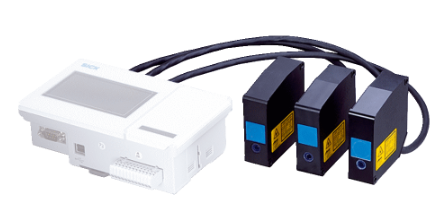
\includegraphics[scale=0.40]{figuras/sensor_SICK_1.png}
        %%\caption{Articulaciones del UR}
        \label{fig:articulaciones_UR}
    \end{subfigure}
    \hfill
    \begin{subfigure}[h!]{0.35\textwidth}
        \begin{tabular}{|l|r|}
            \hline
            Peso & 250 g \\
            \hline
            Rango de medida & 25-35 mm \\
            \hline
            Precisión de repetición & 0.2 $\mu$m \\
            \hline
            Tiempo de respuesta & 0.1-0.8 ms \\
            \hline
        \end{tabular}
        %%\caption{Valores característicos}
        \label{tab:caracteristicas_UR_tabla}
    \end{subfigure}
    \caption{Características del sensor SICK OD5-30W05 \cite{manuel_sensor_laser_sick_od5_30w05}}
    \label{tab:caracteristicas_sensor_sick_od5}
\end{table}

\subsection{Utillaje para el sensor de medida}
El sensor de medida se apoya sobre un utillaje diseñado en trabajos previos \cite{TFM_SanchoAmparo} y mejorado por compañeros del marco de trabajo. Este utillaje sirve como un soporte rígido y estable para ubicar otros elementos en el futuro como puede ser el extrusor de la estación robotizada \acrshort{NPAM}.

Este utillaje también ha servido de referencia para establecer restricciones en el cálculo de trayectorias a partir de su modelo \acrshort{CAD}. Se muestra como referencia la Figura \ref{fig:entorno_virtual_rviz}.

\subsection{Cama de impresión}
La cama de impresión utilizada en este proyecto ha sido elaborada como trabajo de fin de titulación de Iñaki Echepare \cite{TFM_IñakiEchepare}. Se ha utilizado como objetivo de trazado de trayectorias y comprobación de su exactitud. 

De forma análoga al utillaje para el sensor de medida, se implementa su modelo \acrshort{CAD} dentro del entorno virtualizado para establecer una nueva restricción en el cálculo de trayectorias. La Figura muestra una fotografía de la cama real con sus partes más importantes y a su lado su representación en el entorno virtual.

\begin{figure}[h!]
    \centering
    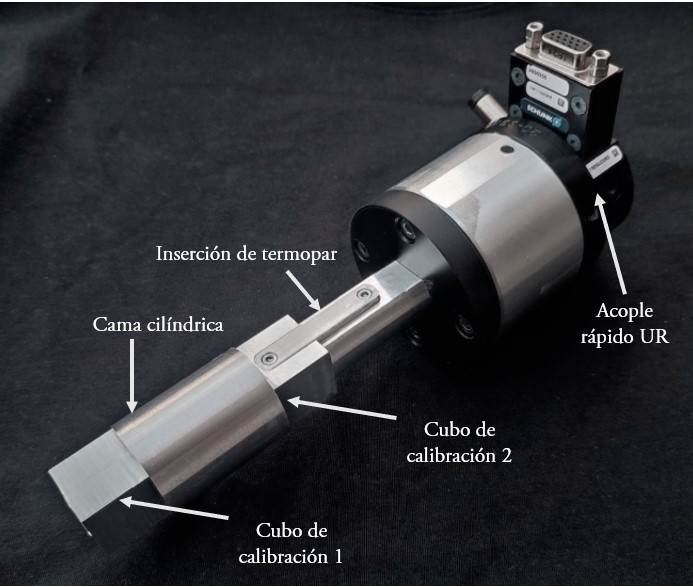
\includegraphics[scale=0.4]{figuras/cama_impresion_real.jpg}
    \label{fig:cama_impresion_real}
    \caption{Cama de impresión \cite{TFM_IñakiEchepare}}
\end{figure}

A continuación se describen algunas de las partes más importantes de la cama:

\begin{itemize}
    \item \textbf{Acople rápido UR:} Elemento de unión y sujeción de la cama al UR.
    \item \textbf{Cubos de calibración:} Dos geometrías diseñadas específicamente para establecer sistemas de referencia y puntos clave que permiten ubicar la cama en el espacio.
    \item \textbf{Cama:} Pieza de revolución (en este caso un cilindro simple) sobre la que se irá depositando el material extruído. En su interior dispone de un cartucho calefactor que proporciona el calor requerido para que el material solidifique de la forma deseada.
    \item \textbf{Inserción termopar:} Pletina de acceso a un dispositivo de medida de temperatura directa del cartucho calefactor.
\end{itemize}

\subsection{Controlador de temperatura}
Sistema de accionamiento del cartucho calefactor de la cama de impresión y lectura de su temperatura. Dispone de un termopar tipo K, un amplificador de la señal del termopar MAX6675 (características principales indicadas en la Tabla \ref{tab:caracteristicas_termopar}), un relé y una placa electrónica con controlador programble. El esquema eléctrico ha sido elaborado por Irene Rodríguez y ha contado con la revisión y control de ensayos del autor del presente proyecto.

\begin{table}[H]
    \centering
       \begin{tabular}{|l|r|}
            \hline
            Resolución & ±0.25 ºC\\
            \hline
            Rango de temperatura & 0-1024 ºCC \\
            \hline
            Tensión de alimentación & 0.3-6 V\\
            \hline
            Intensidad de salida & 50 mA \\
            \hline
            Constante de conversión & 41 $\mu$V/ºC \\
            \hline
            Temperatura de trabajo & 0-50 ºC \\
            \hline
        \end{tabular}
    \caption{Características del termopar MAX6675 \cite{manual_termopar_driver_max6675}}
    \label{tab:caracteristicas_termopar}
\end{table}

